\documentclass[sigconf,nonacm]{acmart}
\settopmatter{printacmref=false, printccs=false, printfolios=true}
\renewcommand\footnotetextcopyrightpermission[1]{}

\acmConference[CompPar '26]{Computa\c{c}\~ao Paralela (CompPar 2026/27)}{November 2026}{FCT NOVA, Caparica, Portugal}
\renewcommand{\shortauthors}{J. Silva and J. Pisco}

\usepackage{booktabs}
\usepackage{graphicx}
\sloppy

\begin{document}
\title{Large-Scale Analytics and Performance Engineering with PySpark on NYC Yellow Taxi Data}

\author{Jo\~ao Silva}
\email{p212794@campus.fct.unl.pt}

\author{Jos\'e Manuel Fernandes Pisco}
\email{p212228@campus.fct.unl.pt}

\begin{abstract}
Writing a PySpark pipeline that produces correct results is fairly straightforward, but making it run fast on a distributed cluster requires understanding where the engine spends its time. In this report, we build and profile an analytical pipeline over the 2020 New York City Yellow Taxi dataset (roughly 24.6 million trips across 12 monthly Parquet files) paired with the official taxi zone lookup table. Our pipeline implements three mandatory tasks---data cleaning, temporal demand analysis, and monthly zone statistics---along with two optional tasks: fare anomaly detection and demand forecasting with a four-week lag. Starting from a naive baseline on a three-worker Docker Spark cluster, we use the Lab~3 profiler and the Spark Web UI to identify bottlenecks and apply four incremental optimisations: caching reused data, pruning unneeded columns during a single unified file scan, broadcasting the small lookup table, and tuning Adaptive Query Execution (AQE) shuffle partitions to prevent disk spilling. Together, these steps cut execution time from 83.61 seconds down to 27.63 seconds (a $3.03\times$ speedup), reduce network shuffle volume by more than half, and eliminate over 400 MB of disk spill. Finally, we test how the tuned pipeline scales with larger data fractions and additional worker nodes.
\end{abstract}

\keywords{Apache Spark, PySpark, Performance Profiling, Adaptive Query Execution, Data Skew, Scalability}

\maketitle

\section{Introduction}

In this project, we work with the NYC Taxi \& Limousine Commission (TLC) Yellow Taxi dataset \cite{nyctlc2026} for the full year of \textbf{2020}, combined with a small 265-row zone lookup CSV file that maps numeric location IDs to borough and zone names. Across all 12 monthly Parquet files, the 2020 dataset takes up 358 MB on disk and contains 24.65 million raw trip records. Our pipeline implements the three mandatory operations---\textbf{M1} (data ingestion and cleaning), \textbf{M2} (hourly and daily demand by borough), and \textbf{M3} (monthly zone statistics with three-month rolling windows)---as well as two optional operations: \textbf{O1} (detecting abnormally high per-mile fares across weekdays and weekends) and \textbf{O3} (computing four-week lag features for demand forecasting).

This workload is particularly interesting from a performance perspective because the data is naturally unbalanced in two ways. First, because the COVID-19 lockdown hit New York in March 2020, the monthly files vary wildly in size: January and February are around 90 MB each (over 6 million trips per month), whereas April is only 4.2 MB (238 thousand trips). Second, taxi traffic is heavily concentrated in Manhattan, which accounts for roughly 60\% of all rides. On top of this skewed data, our two optional tasks push Spark in different ways: \textbf{O1} runs window functions over the entire unaggregated trip table (forcing all 22.7 million clean trips through a single wide shuffle and sort), while \textbf{O3} requires a wide self-join to match each day's traffic with traffic from four weeks earlier.

\section{Pipeline}

We built the pipeline using the PySpark \textbf{DataFrame API} rather than low-level RDDs \cite{pysparkapi2026, sparktuning2026}. As we learned in the lectures and labs, both the DataFrame API and Spark SQL compile down to the exact same physical execution plan through the Catalyst optimizer and the Tungsten execution engine. Using DataFrames allowed us to chain transformations cleanly in Python while still benefiting from automatic predicate pushdown, column pruning, and whole-stage code generation, without paying the heavy serialization penalty of Python user-defined functions (UDFs).

\textbf{M1 --- Data Ingestion and Cleaning.} We read the monthly Parquet files, cast all columns to their expected types, and drop incomplete rows containing null values (which removes about 810k rows, mostly missing passenger counts). We then count how many records violate each of the five validity rules (shown in Table~\ref{tab:m1_stats}) and filter them out, leaving 22.68 million valid trips for the rest of the pipeline.

\textbf{M2 --- Temporal Demand Analysis.} We join the cleaned trips with the zone lookup table to get the pickup borough, extract the day of the week and hour of the day, and calculate trip duration in minutes from the pickup and dropoff timestamps. We then group by borough, day, and hour to compute total trips and average fare, duration, and distance, saving the result as Parquet partitioned by borough.

\textbf{M3 --- Zone-Level Statistics.} We aggregate trips by pickup zone and month to get monthly volume and the mean and standard deviation of fare and distance. Using window functions, we rank zones by volume inside each borough, compute each zone's rolling three-month share of borough traffic, and flag months where a zone's volume deviates from its rolling three-month average by more than 1.5 standard deviations.

\textbf{O1 --- Fare Anomaly Detection.} Using a window partitioned by pickup zone and hour of the day over the full trip table, we calculate the mean and standard deviation of the fare per mile for every trip. Trips exceeding the bucket mean plus three standard deviations are flagged as anomalies. We then group by borough and payment type and pivot the results to compare weekday versus weekend anomaly rates.

\textbf{O3 --- Demand Forecasting Features.} We first count trips per zone, date, day of the week, and hour. To get the four-week lag without scanning the raw trips twice, we create a second view of these daily counts with the date shifted forward by 28 days and left-join the two tables together. Finally, we use a window over each zone, weekday, and hour to compute the historical mean and variance, flag hours where demand is more than double the historical average, and join the lookup table to attach the service zone.

\begin{table}[t]
\centering
\caption{M1 cleaning statistics on the 2020 dataset (after dropping null rows). A few stray rows had corrupted years.}
\label{tab:m1_stats}
\vspace{-0.15cm}
\resizebox{\columnwidth}{!}{%
\begin{tabular}{lrrrrrr}
\toprule
\textbf{Year} & \textbf{Non-Null} & \textbf{Fare $\le 0$} & \textbf{Dist $\le 0$} & \textbf{Pass $\notin [1,6]$} & \textbf{Drop $\le$ Pick} & \textbf{Zone $\notin [1,263]$} \\
\midrule
2020 & 23,838,845 & 103,249 & 317,571 & 489,585 & 15,802 & 266,363 \\
Other & 280 & 20 & 28 & 0 & 0 & 7 \\
\bottomrule
\end{tabular}%
}
\vspace{-0.2cm}
\end{table}

\paragraph{Physical Execution Plan.}
Figure~\ref{fig:exec_plan} shows a simplified diagram of the physical plan for \textbf{M2} before and after our optimisations. In the baseline plan (left), Spark treats the 265-row CSV lookup table like a large dataset, shuffling and sorting all 22.7 million taxi trips across 200 partitions just to perform a sort-merge join. In the optimised plan (right), the cleaned trips are read directly from memory cache and joined with a broadcast copy of the lookup table, completely avoiding the shuffle and sort on the trip data.

\begin{figure}[h]
\centering
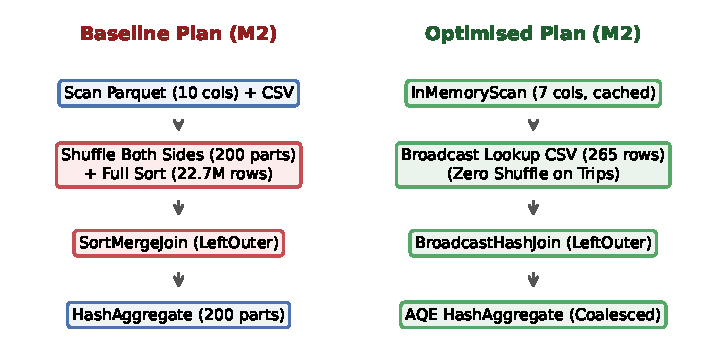
\includegraphics[width=0.98\columnwidth]{figures/fig0_execution_plan.pdf}
\vspace{-0.2cm}
\caption{Simplified physical execution plan for M2 (baseline sort-merge join vs.\ optimised broadcast join).}
\label{fig:exec_plan}
\vspace{-0.2cm}
\end{figure}

\section{Profiling and Baseline}

\paragraph{Experimental Setup.}
We ran all benchmarks on a Linux machine (16 logical CPU cores, 23 GiB RAM) using the course Docker cluster running \textbf{Apache Spark 4.2.0}. For our baseline and optimisation experiments, the cluster was configured with one master node, \textbf{three worker containers} (2 CPU cores and 2 GB of RAM per worker, giving 6 executor cores and $3 \times 1.5\text{ GB} = 4.5\text{ GB}$ of total executor heap), and one driver container (2 GB of RAM). We used the Lab~3 profiler helper to record stage metrics and queried the Spark UI REST API \cite{sparkmonitoring2026} to measure task duration skew.

\paragraph{Baseline Results and Bottlenecks.}
To get a true unoptimised baseline (\texttt{0-baseline}), we ran the pipeline with Adaptive Query Execution turned off, default shuffle partitions set to 200, no caching, and automatic broadcast joins disabled. As shown in Table~\ref{tab:opt_summary} and Figure~\ref{fig:opt_study}, the baseline took \textbf{83.61 seconds}, launched \textbf{7,681 tasks} across 78 stages, and shuffled \textbf{1.30 GB} of data across the network. Looking at the Spark UI and execution plans pointed to four clear bottlenecks.

\textbf{1. Repeated File Reads.} Because nothing was cached after M1, Spark went back to disk and re-read all 12 Parquet files from scratch \textbf{six separate times} (once for M1, M2, M3, and O1, and twice for the two sides of the self-join in O3).

\textbf{2. Uneven File Scans and Extra Columns.} Reading the 12 monthly files separately and unioning them created 57 tasks per scan with huge load imbalance. In Stage~107, the median task finished in \textbf{56 ms}, while the slowest task (scanning January 2020) took \textbf{10,009 ms}---\textbf{$178.7\times$ the median}! We were also keeping columns like tip amount, total amount, and dropoff location ID that were never used after M1.

\textbf{3. Unnecessary Join Shuffles.} Joining the trip table with the tiny 265-row zone table via sort-merge joins forced Spark to shuffle and sort millions of rows four separate times, creating over half of our 1.30 GB shuffle traffic.

\textbf{4. Too Many Small Tasks and Skewed Shuffles.} Using 200 fixed shuffle partitions on a 6-core cluster created thousands of tiny tasks. Worse, because Manhattan dominates trip volume, shuffle stages were heavily skewed: in Stage~136 (200 tasks), the median task took \textbf{21 ms} while the slowest task took \textbf{2,738 ms} (\textbf{$130.4\times$ the median}).

\section{Optimisation Study}

Following the Lab~3 methodology (\emph{profile $\to$ hypothesise $\to$ optimise $\to$ measure}), we applied one fix at a time and measured its cumulative impact on the 3-worker cluster (Figure~\ref{fig:opt_study} and Table~\ref{tab:opt_summary}).

\begin{figure*}[t]
\centering
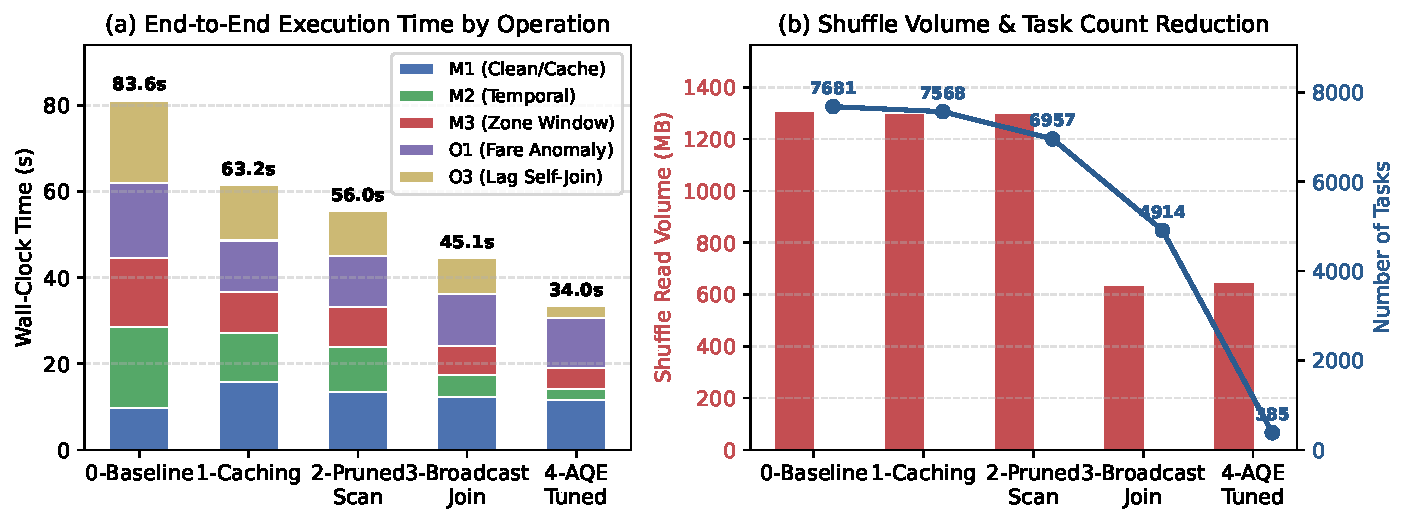
\includegraphics[width=0.95\textwidth]{figures/fig1_optimisation_study.pdf}
\vspace{-0.25cm}
\caption{Step-by-step optimisation progression on the 3-worker cluster (full 2020 dataset, 23.8M records): (a) stacked wall-clock time per operation, and (b) shuffle read volume (MB) and total task count.}
\label{fig:opt_study}
\vspace{-0.15cm}
\end{figure*}

\subsection{Opt 1: Caching Reused DataFrames}
\textbf{(a) Bottleneck:} The baseline scanned and filtered the raw Parquet files six times across the pipeline because Spark recomputes lazy transformations on every action.
\textbf{(b) Hypothesis:} Caching the cleaned trips after M1 (and caching the daily-hourly counts before the self-join in O3) will let M2, M3, O1, and O3 read directly from memory instead of disk.
\textbf{(c) Change:} We cached the cleaned trip table after M1 and the aggregated bucket table in O3, unpersisting both at the end of the run.
\textbf{(d) Result:} End-to-end wall time dropped from \textbf{83.61 s to 63.25 s ($-24.4\%$)}, and total executor runtime fell from 350.1 s to 268.6 s. Although M1 took about 6 seconds longer to materialise the cache, every downstream operation sped up by 5 to 7 seconds (Figure~\ref{fig:opt_study}a).

\subsection{Opt 2: Unified File Scan and Column Pruning}
\textbf{(a) Bottleneck:} Reading the 12 monthly files in a loop and unioning them produced 57 skewed tasks per scan, and caching 10 columns when only 7 were needed wasted executor memory, causing 69.1 MB of disk spill.
\textbf{(b) Hypothesis:} Passing all 12 files to a single Parquet read allows Spark to pack them into balanced partitions, and dropping the three unused columns before caching reduces memory pressure.
\textbf{(c) Change:} We replaced the 12-file union loop with a single vectorized Parquet read (which packed the data into 7 balanced partitions) and dropped the unused columns.
\textbf{(d) Result:} Wall time dropped further from \textbf{63.25 s to 55.97 s ($-11.5\%$ vs.\ Opt~1)}, the cached memory footprint read by downstream stages shrank by 34.6\% (from 4.67 GB to 3.05 GB), and the number of stages fell from 77 to 66.

\subsection{Opt 3: Broadcast Hash Joins}
\textbf{(a) Bottleneck:} Even with caching and column pruning, the pipeline still shuffled 1.29 GB of data because M2, M3, O1, and O3 used sort-merge joins for the 265-row zone lookup table.
\textbf{(b) Hypothesis:} Since the zone lookup table is only 13 KB on disk, broadcasting a copy to every worker will replace all four sort-merge joins with local hash lookups, avoiding any shuffle of the trip data during joins.
\textbf{(c) Change:} We added an explicit broadcast hint to the pickup zone lookup table in M2, M3, O1, and O3.
\textbf{(d) Result:} Network shuffle volume was cut in half---\textbf{dropping by 51.3\% from 1,293.2 MB to 629.4 MB} (Figure~\ref{fig:opt_study}b). Total stages dropped from 66 to 47, disk spill dropped to zero, and wall time fell from \textbf{55.97 s to 45.06 s ($-19.5\%$ vs.\ Opt~2)}, with M2 alone dropping from 10.47 s to 5.07 s.

\subsection{Opt 4: Adaptive Query Execution and Partition Sizing}
\textbf{(a) Bottleneck:} After Opt~3, all remaining shuffles were wide aggregations and windows, which still used 200 fixed partitions (4,914 tasks total) and suffered from heavy skew ($117.7\times$ max-to-median task time ratio in O1).
\textbf{(b) Hypothesis:} Enabling Adaptive Query Execution (AQE) \cite{sparktuning2026}---including partition coalescing, skew-join handling, and the local shuffle reader---along with tuning the shuffle partition count will eliminate tiny-task overhead and balance skewed stages.
\textbf{(c) Change and Spill Discovery:} We first enabled AQE with a 16 MB target partition size and lowered shuffle partitions from 200 to 12 ($2 \times$ our 6 cluster cores, labelled \texttt{4a-aqe-12} in Table~\ref{tab:opt_summary}). This cut total tasks by \textbf{95.0\% (from 7,681 to 385)}, reduced O1's shuffle task skew from \textbf{$130.4\times$ down to just $1.17\times$}, and lowered wall time to \textbf{33.95 s}. However, the profiler caught an important problem: forcing O1's 644 MB shuffle into only 12 partitions made each partition too big to sort inside the remaining executor memory, causing \textbf{1.5 GB of memory spill and 406.7 MB of disk spill}! Because AQE can merge small partitions but cannot split an already oversized window partition, we increased the initial shuffle partitions to \textbf{48} (\texttt{4b-aqe-48}).
\textbf{(d) Result:} With 48 initial partitions, AQE still merged the small shuffles in M2, M3, and O3 down to 4--12 tasks, while keeping O1 spread across 48 smaller ($\approx 13\text{ MB}$) partitions. This \textbf{completely eliminated all disk spill (0.0 MB)} and brought our final execution time down to \textbf{27.63 s}---a \textbf{$3.03\times$ overall speedup} over the baseline.

\begin{table}[t]
\centering
\caption{Summary of all optimisations on the 3-worker cluster (6 cores, full 2020 dataset).}
\label{tab:opt_summary}
\vspace{-0.15cm}
\footnotesize
\setlength{\tabcolsep}{2.5pt}
\begin{tabular}{lrrrrrr}
\toprule
\textbf{Run} & \textbf{Time (s)} & \textbf{Speedup} & \textbf{Stages} & \textbf{Tasks} & \textbf{Shuf (MB)} & \textbf{Spill (MB)} \\
\midrule
\texttt{0-baseline} & 83.61 & $1.00\times$ & 78 & 7,681 & 1,303.3 & 0.0 \\
\texttt{1-caching} & 63.25 & $1.32\times$ & 77 & 7,568 & 1,293.7 & 69.1 \\
\texttt{2-pruned-scan} & 55.97 & $1.49\times$ & 66 & 6,957 & 1,293.2 & 55.2 \\
\texttt{3-broadcast} & 45.06 & $1.86\times$ & 47 & 4,914 & 629.4 & 0.0 \\
\texttt{4a-aqe-12} & 33.95 & $2.46\times$ & 76 & 385 & 644.2 & 406.7 \\
\texttt{4b-aqe-48} & \textbf{27.63} & \textbf{$3.03\times$} & 67 & 816 & \textbf{631.2} & \textbf{0.0} \\
\bottomrule
\end{tabular}
\vspace{-0.2cm}
\end{table}

\section{Analysis}

\begin{figure*}[t]
\centering
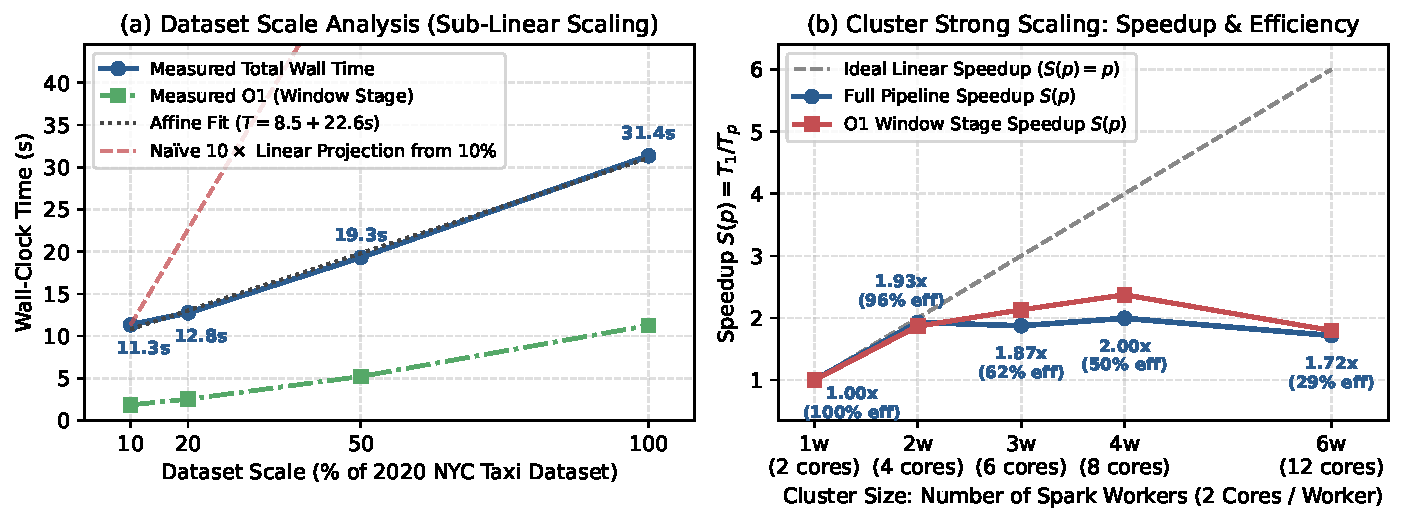
\includegraphics[width=0.95\textwidth]{figures/fig2_scalability_analysis.pdf}
\vspace{-0.25cm}
\caption{Scalability analysis of the optimised pipeline: (a) execution time vs.\ dataset fraction on 3 workers, and (b) strong-scaling speedup $S(p) = T_1 / T_p$ and parallel efficiency $E(p) = S(p)/p$ from 1 to 6 workers.}
\label{fig:scalability}
\vspace{-0.15cm}
\end{figure*}

\paragraph{1. Dataset Scale (10\% to 100\%).}
To see how our tuned pipeline handles growing data volumes, we ran it on 10\%, 20\%, 50\%, and 100\% samples of the 2020 dataset on the 3-worker cluster (Figure~\ref{fig:scalability}a). Increasing the dataset size by $10\times$ (from 10\% to 100\%) only increased total runtime by \textbf{$2.77\times$} (from 11.33 s to 31.35 s). In other words, execution time scales \textbf{sub-linearly}. As shown by the dotted fit line in Figure~\ref{fig:scalability}a, every run has a fixed baseline cost of about 8.5 seconds (spent reading file metadata, planning 34 Spark jobs, and broadcasting the lookup table), plus a variable cost of about 22.6 seconds that grows linearly with the data. This matches \textbf{Gustafson-Barsis' Law} as covered in parallel computing theory (Lecture~7): as the dataset grows, the fixed sequential overhead becomes a much smaller fraction of the total runtime, allowing the cluster to use its parallel cores more efficiently. Looking at individual tasks, the heavy window sort in \textbf{O1} (green curve in Figure~\ref{fig:scalability}a) scales almost purely linearly with data size because shuffle volume grows proportionally from 75.5 MB at 10\% to 644.2 MB at 100\%.

\paragraph{2. Cluster Size Strong Scaling (1 to 6 Workers and Local Mode).}
Next, we kept the full 100\% dataset fixed and scaled the cluster across 1, 2, 3, 4, and 6 workers (2 to 12 cores), as well as local mode with 4 and 16 threads on the host machine (Figure~\ref{fig:scalability}b and Table~\ref{tab:cluster_scale}).
\begin{table}[b]
\centering
\caption{Strong scaling on the full 2020 dataset using the Lecture~7 metrics: Speedup $S(p) = T_1/T_p$ and Efficiency $E(p) = S(p)/p$.}
\label{tab:cluster_scale}
\vspace{-0.15cm}
\small
\setlength{\tabcolsep}{4pt}
\begin{tabular}{lrrrrrr}
\toprule
\textbf{Config} & \textbf{Cores} & \textbf{$T_p$ (s)} & \textbf{$S(p)$} & \textbf{$E(p)$} & \textbf{O1 (s)} & \textbf{Spill (MB)} \\
\midrule
1 Worker (\texttt{1w}) & 2 & 65.20 & $1.00\times$ & 100.0\% & 25.42 & 513 \\
2 Workers (\texttt{2w}) & 4 & 33.82 & $1.93\times$ & 96.4\% & 13.61 & 372 \\
3 Workers (\texttt{3w}) & 6 & 34.78 & $1.87\times$ & 62.5\% & 11.93 & 444 \\
4 Workers (\texttt{4w}) & 8 & 32.67 & $2.00\times$ & 49.9\% & 10.71 & 291 \\
6 Workers (\texttt{6w}) & 12 & 37.97 & $1.72\times$ & 28.6\% & 14.14 & 82 \\
\midrule
\texttt{local[4]} & 4 & 35.18 & $1.85\times$ & --- & 14.72 & 516 \\
\texttt{local[*]} & 16 & 32.59 & $2.00\times$ & --- & 10.19 & 531 \\
\bottomrule
\end{tabular}
\end{table}
Doubling the cluster from 1 to 2 workers (2 to 4 cores) gave a nearly ideal speedup of \textbf{$1.93\times$ ($96.4\%$ efficiency)}. Beyond 2 workers, however, total pipeline speedup plateaued around $2.00\times$ at 4 workers ($50\%$ efficiency) and dropped to $1.72\times$ at 6 workers, even though the window stage \textbf{O1} continued scaling up to $2.37\times$ at 4 workers (red curve in Figure~\ref{fig:scalability}b). The theoretical models from Lecture~7 (\textbf{Amdahl's Law} and the \textbf{DAG Work-Span model}) explain both effects.

\textbf{Critical-Path Span Limit in M1.} When Spark scans the 12 Parquet files using its default 128 MB split size, it creates 7 partitions. Because pre-lockdown January (90 MB, 6.4M rows) and February (88 MB, 6.3M rows) each fit inside a single 128 MB split, \textbf{just two partitions hold 53\% of the entire year's data}. In the Work-Span model, a stage can never finish faster than its longest single task (the span $T_\infty \approx 11\text{ s}$ to scan and cache January), which caps the effective parallelism of M1 at $23.8\text{M} / 6.4\text{M} \approx 3.7$ cores. Once we reach 2 workers (4 cores), two cores are busy scanning January and February while any additional cores finish the tiny spring/summer months in 2 seconds and sit idle waiting for the stage barrier.

\textbf{Memory Relief vs.\ Shuffle Contention at 6 Workers and Local Mode.} Adding more workers increases total cluster memory (from 1.5 GB at 1 worker to 9.0 GB at 6 workers), which steadily reduces disk spill by 84\% (from 513 MB down to 82 MB in Table~\ref{tab:cluster_scale}). However, because all 6 worker containers run on the same host machine, going from 4 to 6 workers increases virtual network and disk contention across $6 \times 6 = 36$ shuffle streams, increasing non-CPU wait time from 7.5 s to 26.7 s. Similarly, running \texttt{local[*]} with 16 threads inside a single 2 GB JVM caused heavy garbage collection pauses (49.4 s of non-CPU wait time).

\section{Discussion}

\paragraph{Remaining Bottlenecks.}
Two main bottlenecks remain in our final pipeline: (1) M1's initial scan is limited by the two large pre-lockdown monthly files (we tested lowering the maximum file split size to 16 MB to force 26 even splits, which balanced M1 but created extra task overhead in later stages), and (2) \textbf{O1} still takes about 40\% of total runtime because computing window functions over every individual ride requires sorting all 22.7 million rows.

\paragraph{Limitations of Methodology.}
Because our cluster runs inside Docker containers on a single machine, all workers compete for the same physical SSD and memory bus. On a real multi-server cluster where each node has its own disk and network card, 4 and 6 workers would not suffer the same I/O contention we observed here.

\paragraph{What We Would Do With More Time.}
With more time, we would replace the full-table window in \textbf{O1} with a standard \texttt{groupBy} aggregation to compute the mean and standard deviation for each of the $263 \times 24 = 6{,}312$ zone-hour buckets, and then broadcast-join that tiny 6,312-row summary table back to the main trip table. That simple algorithmic change would compute the exact same result while avoiding the 631 MB window sort altogether.

\clearpage
\section*{Extra Page: Bibliography, Acknowledgements \& Contributions}

\bibliographystyle{acm}
\bibliography{refs}

\section*{Acknowledgements}
We thank Professor Herv\'e Paulino for providing the Lab~3 profiler tool and for the tips on tuning Adaptive Query Execution and shuffle partition sizes for skewed datasets.

\textbf{Use of AI Tools:} In line with the assignment guidelines, AI assistants (GitHub Copilot / LLM assistant) were used to help write the automated benchmark script (\texttt{run\_benchmarks.py}), generate the Matplotlib plotting script (\texttt{generate\_plots.py}), and format the LaTeX tables. All PySpark queries, profiling experiments, and performance conclusions were tested and verified on our Docker Spark cluster.

\section*{Individual Contributions}
\begin{table}[h]
\centering
\begin{tabular}{llp{4.0cm}}
\toprule
\textbf{Member} & \textbf{Share} & \textbf{Main Responsibilities} \\
\midrule
Jo\~ao Silva & 50\% & Standalone CLI script, O3 self-join implementation, AQE and partition tuning, scalability benchmarks, and Sections 4--6 of the report. \\
Jos\'e Manuel Fernandes Pisco & 50\% & Initial Jupyter notebook, M1--M3 and O1 DataFrame/Window queries, Docker cluster setup, and Sections 1--3 of the report. \\
\bottomrule
\end{tabular}
\end{table}

\section*{Comments and Suggestions}
The Lab~3 profiler made it much easier to compare before-and-after metrics without manually copying numbers from the Spark UI. Working with the full 2020 dataset (358 MB) was also a great size for local cluster testing: large enough to trigger real 1.3 GB shuffles, 400 MB disk spills, and $130\times$ task skew, while still finishing in under a minute once tuned.

\end{document}
